\section{Introduction}
The study of Supersymmetry provides a fruitful playground for physicists to test various aspects of  physics beyond the Standard Model (BSM) ranging from Early Universe Cosmology and Dark Matter to modern theoretical frameworks such as String Theory or the AdS/CFT-correspondence.\\
At the end of the first part of our talk we concluded the discussion of the theoretical foundations of the MSSM with a parameter count that left us with the unsatisfying observation that one would need to determine 124 independent parameters in total to fully characterize the model. Such a large amount of relevant parameters makes the MSSM not phenomenologically viable \cite{MSSMGroup1998}.\\
The phenomenology of the MSSM is to a large extend determined by the SUSY breaking mechanism and the associated SUSY breaking scale \cite{PDG20182019}. We will motivate phenomenological constraints we want to put on the MSSM and see how they are implemented technically. Additionally we want to highlight the (possible) importance of gravity at high energies. This will help us to reduce the number of relevant parameters and may provide a starting point for actual experimental tests. For a schematic overview of the main concepts we want to discuss, have a look at Figure \ref{fig:roadmap} at the beginning of the next page.

\begin{figure}[t]
\centering
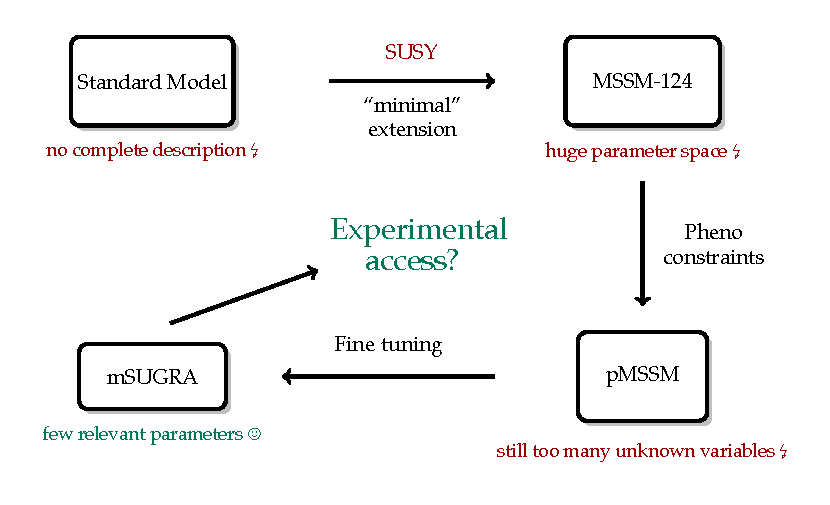
\includegraphics{figures/overview}
\caption{Schematic overview of the \enquote{roadmap} of our talk.}
\label{fig:roadmap}
\end{figure}
\newpage